\documentclass{article}
\usepackage{hyperref}
\usepackage{graphics}
\usepackage{graphicx}
\newcommand{\Rfunction}[1]{{\texttt{#1}}}
\newcommand{\Robject}[1]{{\texttt{#1}}}
\newcommand{\Rpackage}[1]{{\textit{#1}}}

\usepackage{/Library/Frameworks/R.framework/Resources/share/texmf/Sweave}
\begin{document}
\title{Inferring mutual information networks using the \Rpackage{minet} package}
\author{Patrick E. Meyer, Fr\'ed\'eric Lafitte, Gianluca Bontempi}
%\VignetteIndexEntry{Inferring mutual information networks using the minet package}
\maketitle
%____________________________________________________________________________________________________________________________INTRODUCTION
\section{Introduction}

Two important issues in computational biology are the extent to      
which it is possible to model transcriptional interactions by large   
networks of interacting elements and how these interactions can be  
effectively learned from measured expression data \cite{vansomeren}. It should     
be noted that by focusing only on transcript data, the inferred     
network should not be considered as a proper biochemical regulatory 
network, but rather as a gene-to-gene network where many     
physical connections between macromolecules might be hidden by
short-cuts. In spite of some evident limitations the bioinformatics
 community made important advances in this domain over the
last few years \cite{gardner,schafer}. In particular, mutual information networks
have been succesfully applied to transcriptional network inference
\cite{aracne,clr}. Such methods, which typically rely on the estimation of
mutual information between variables, have recently held the attention
 of the bioinformatics community for the inference of very large
networks \cite{relnet,aracne,clr,papier}.

The \Rpackage{minet} package provides a set of functions to infer 
mutual information networks from a dataset. If fed with microarray 
data, the package returns a network where nodes denote genes and 
edges model statistical dependencies between genes. 
The weight of an edge provides evidence about the existence 
of a specific (e.g transcriptional) gene to gene interaction. 

The inference proceeds in two steps. First, the Mutual Information
Matrix ($MIM$) is computed, a  square matrix whose $MIM_{ij}$ term is the mutual 
information between gene $X_i$ and $X_j$. Secondly, an inference algorithm
takes the $MIM$ matrix as input and attributes a score to each edge
connecting a pair of nodes. Different entropy estimators are implemented 
in this package as well as different inference methods, namely
\Robject{aracne}, \Robject{clr} and \Robject{mrnet} \cite{aracne,clr,papier}. 
Also, the package integrates accuracy assessment tools, like PR-curves and ROC-curves, 
to compare the inferred network with a reference one.

This vignette guides the package user in :
\begin{enumerate}
\item Estimating the mutual information matrix and discretizing data if needed.
\item Inferring a network modeling the interactions between the dataset's variables.
\item Comparing the infered network to a network of known interactions in order to compute $F_\beta-scores$.
\item Plotting precision-recall and receiver operating characteristic curves.
\item Plotting the infered network using the \Rpackage{Rgraphviz} package. 
\end{enumerate}

The data used in the following examples was generated using the {\it SynTReN}
simulator \cite{syntren}. This data generator uses a known network of interacting genes
in order to generate gene expression levels for all the genes included in the network. 
Once the network is infered from the generated data, it can be compared to the true 
underlying network in order to validate the inference algorithm. 
%___________________________________________________________________________________________________________________MUTUAL INFORMATION ESTIMATION
\section{Mutual Information Estimation}
Mutual information networks are a subcategory of network inference methods.
These methods set a link between two nodes if it exhibits a high score based on
the mutual information between the nodes. 

Mutual informaton networks rely on the computation of the mutual information 
matrix (MIM), a square matrix whose element 
$$ MIM_{ij} = I(X_i ; X_j ) = \sum_{ x_i \in \mathcal{X}_i} \sum_{ x_j\in\mathcal{X}_j} p(x_i , x_j ) \log p(x_i )p(x_j ) $$
is the mutual information between $X_i$ and $X_j$ , where $X_i \in \mathcal{X} ,i = 1, . . . , n$, 
is a discrete random variable denoting the expression level of the \emph{ith} gene.

\subsection{Obtaining The Mutual Information Matrix}
\begin{Schunk}
\begin{Sinput}
> library(minet)
> data(syn.data)
> estimator = "mi.empirical"
> mim <- build.mim(syn.data, estimator)
> mim[1:5, 1:5]
\end{Sinput}
\begin{Soutput}
            CDC11    SWI4   CDC10   SPT16 SWI4_SWI6
CDC11     0.00000 4.60517 4.60517 4.60517   4.60517
SWI4      4.60517 0.00000 4.60517 4.60517   4.60517
CDC10     4.60517 4.60517 0.00000 4.60517   4.60517
SPT16     4.60517 4.60517 4.60517 0.00000   4.60517
SWI4_SWI6 4.60517 4.60517 4.60517 4.60517   0.00000
\end{Soutput}
\end{Schunk}
In the above code, the mutual information matrix is built using the function 
\Rfunction{build.mim}. This function takes the dataset and one of the mutual 
information estimator explained in this section as input. All the estimators require discrete data values. The \Rfunction{discretize} function 
allows the user to choose between two binning
algorithms.
 
\subsection{Supervized Discretization}

All the mutual information estimators described in this section require discrete data values.
If the random variable $X$ is continuous and can take values comprised between
$a$ and $b$, it is always possible to divide the interval $[a, b]$ into $|\mathcal{X}|$ subintervals
in view of using the discrete estimators.
The package provides a function that discretizes data using the equal frequency or equal width
binning algorithm \cite{discretize}.

\subsubsection{Equal Width Binning}
The principle of the equal width discretization is to divide $[a, b]$ into $|\mathcal{X}|$ 
subintervals all having the same size: 
$$ [a, a + \frac{b-a}{\mathcal{X}} [, [a + \frac{b-a}{\mathcal{X}} , a + 2 \frac{b-a}{\mathcal{X}} [, ... , [a + (|\mathcal{X} |-1)\frac{b-a}{\mathcal{X}},b + \epsilon[ $$ 
Note that an $\epsilon$ is added in the last interval in order to include the maximal value in one of the 
$|\mathcal{X}|$ bins. This discretization scheme can be done in $O(m)$.
\begin{Schunk}
\begin{Sinput}
> library(minet)
> data(syn.data)
> disc <- "equalwidth"
> nbins <- sqrt(nrow(syn.data))
> ew.data <- discretize(syn.data, disc, nbins)
> syn.data[1:5, 1:5]
\end{Sinput}
\begin{Soutput}
      CDC11      SWI4     CDC10     SPT16 SWI4_SWI6
1 0.4916395 0.2687357 0.5736381 0.2119972 0.2599864
2 0.8342323 0.6566324 0.8750186 0.2810182 0.6977198
3 0.8208405 0.6351676 0.8643861 0.4749119 0.6726126
4 0.9841594 0.9593638 0.9885627 0.9474643 0.9674964
5 0.9879920 0.9690066 0.9913392 0.9999866 0.9764548
\end{Soutput}
\begin{Sinput}
> ew.data[1:5, 1:5]
\end{Sinput}
\begin{Soutput}
  CDC11 SWI4 CDC10 SPT16 SWI4_SWI6
1     2    1     2     2         0
2     7    6     7     2         6
3     7    5     7     4         6
4     9    9     9     9         9
5     9    9     9     9         9
\end{Soutput}
\end{Schunk}
\subsubsection{Equal Frequencies Binning}
The equal frequency discretization scheme consist in dividing the interval $[a, b]$
into $|\mathcal{X}|$ intervals, each having the same number of data points (i.e., 
$\frac{m}{|\mathcal{X}|}$ points).
As a result, the size of each interval can be different. Note that if the $| \mathcal{X} |$
intervals have equal frequencies, the computation of entropy is straightforward since
it is log $\frac{ 1 }{ | \mathcal{X} | }$ . However, there can be more than $\frac{m}{|\mathcal{X}|}$ 
identical values in a vector of measurements. In the latter case, one of the bins will have more 
points than the others and the entropy will be different from $\frac{1}{|\mathcal{X}|}$.
\begin{Schunk}
\begin{Sinput}
> disc <- "equalfreq"
> ef.data <- discretize(syn.data, disc, nbins)
> ef.data[1:5, 1:5]
\end{Sinput}
\begin{Soutput}
  CDC11 SWI4 CDC10 SPT16 SWI4_SWI6
1     0    0     0     1         0
2     4    4     4     1         4
3     3    3     3     4         3
4     9    9     9     9         9
5     9    9     9     9         9
\end{Soutput}
\end{Schunk}

\subsection{Mutual Information Estimators}
The package implements four estimators, called \Robject{"mi.empirical"},\Robject{"mi.mm"},
\Robject{"mi.sg"} and \Robject{"mi.shrink"}. 

\subsubsection{Empirical Estimation}
The estimation of mutual information relies on the estimation of entropy as suggested by the following formula:
$$I(X;Y) = H(X) + H(Y) - H(X,Y)$$ where
$$H(X) = - \sum_{x \in \mathcal{X}} p(x) \log(p(x)) $$
is the entropy of the discrete variable $X$.
The empirical estimator (also called "plug-in", "maximum likelihood" or "naive",
see [29]) is simply the entropy of the empirical distribution:
$$\hat{H}^{emp}(p(X))=-\sum_{i\in\mathcal{X}}\frac{nb(x_{i})}{m}\log\frac{nb(x_{i})}{m}$$
where $nb(x_{i})$ is the counting of data points in bin $x_{i}$.

\subsubsection{Miller-Madow Estimation}
The Miller-Madow estimation is given by the following formula which
is the empirical entropy corrected by the asymptotic bias:
$$\hat{H}^{mm}(p(X)) = \hat{H}^{emp}(p(X)) + \frac{|\mathcal{X}|-1}{2m} $$
where $|\mathcal{X}|$ is the number of bins with non-zero probability. This correction
adds no additional computational cost to the empirical estimator. However, it
reduces the bias without decreasing variance. As a result, it is often preferred
to use the Miller-Madow estimator instead of the empirical entropy estimator.

\subsubsection{Schurmann-Grassberger Estimation}
The Dirichlet distribution is the multivariate generalization of the
beta distribution. It is also the conjugate prior of the multinomial
distribution in Bayesian statistics. More precisely, the density of
a Dirichlet distribution takes the following form
$$f(X;\beta)=\frac{\prod_{i\in\mathcal{X}}\Gamma(\beta_{i})}{\Gamma(\sum_{i\in\mathcal{X}}\beta_{i})}\prod_{i\in\mathcal{X}}x_{i}^{\beta_{i}-1}$$
where $\beta_{i}$ is the prior probability of an event $x_{i}$ and
$\Gamma(\cdot)$ is the gamma function, (see \cite{hausser,nemenman}
for more details).

In front of no apriori knowledge, the $\beta_{i}$ are all set to
equality ($\beta_{i}=N,\ i\in\mathcal{X}$) so as no event becomes
more probable than another. Note that using a Dirichlet prior with
parameters $N$ is equivalent to adding $N\geq0$ \textquotedblleft{}pseudo-counts\textquotedblright{}
to each bin $i\in\mathcal{X}$. The prior actually provides the estimator
the information that $|\mathcal{X}|N$ counts have been observed in
previous experiments. From that viewpoint, $|\mathcal{X}|N$ becomes
the a priori sample size. 

The entropy of a Dirichlet distribution can be computed directly with the following equation:
$$\hat{H}^{dir}(X)=\frac{1}{m+|\mathcal{X}|N}\sum_{i\in\mathcal{X}}(nb(x_{i})+N)(\psi(m+|\mathcal{X}|N+1)-\psi(nb(x_{i})+N+1))$$
where $\psi(z)=\frac{d\ln\Gamma(z)}{dz}$ is the digamma function.

Various choice of prior parameters has been proposed in the literature. 
The Schurmann-Grassberger sets $N=\frac{1}{|\mathcal{X}|}$. 

\subsubsection{Shrinkage Estimation}
Another interesting approach was proposed in \cite{hausser}. The
latter is a shrinkage estimation of the entropy. It proposes to assign
to an event $x_{i}$ a mixture of two probability estimators: 

$$\hat{p}(x_{i})=\lambda\frac{1}{|\mathcal{X}|}+(1-\lambda)\frac{nb(x_{i})}{m}$$

The first one, $\frac{1}{|\mathcal{X}|}$, that has a zero variance
but a large bias and the second one, the empirical one $\frac{nb(x_{i})}{m}$,
that has a larger variance but is unbiased. The advantage of shrinking
the second one towards the first one is that, the resulting estimator
outperform both individual estimates \cite{schafer}.
As the value of $\lambda$ tends to one, the estimated entropy is
moved toward the maximal entropy (uniform probability) whereas when
$\lambda$ is zero the estimated entropy tends to the value of the
empirical one. 

The parameter $\lambda$ has to be chosen in order to minimize a risk
function $R(\lambda)$.

$$R(\lambda)=E[\sum_{i\in\mathcal{X}}(\hat{p}(x_{i})-p(x_{i}))^{2}]$$

In \cite{schafer} the analytical value of $\lambda$
that minimize the risk is expressed in generic terms. Applied to the
problem of estimating bin probabilities \cite{hausser}, it gives
$$\lambda*=\frac{|\mathcal{X}|(m^{2}-\sum_{i\in\mathcal{X}}nb(x_{i})^{2})}{(m-1)(|\mathcal{X}|\sum_{i\in\mathcal{X}}nb(x_{i})^{2}-m^{2})}$$

The entropy can then be computed using
$$\hat{H}^{shrink}=H(\hat{p}(X))=-\sum_{i\in\mathcal{X}}\hat{p}(x_{i})\log\hat{p}(x_{i})$$



%_________________________________________________________________________________________________________________________________NETWORK INFERENCE
\section{Network Inference}
Three network inference methods are available in the package : \Rfunction{aracne}, 
\Rfunction{clr} and \Rfunction{mrnet}. These receive as input the mutual information 
matrix and return the weighted adjacency matrix of the network. The network can be 
directly infered from the dataset by using the \Rfunction{minet} function. This
function takes as input the dataset, the name of the estimator and the name of 
the discretization method to be used as well as the number of bins to be used.

\subsection{Obtaining The Network}
In the following code, the \Rfunction{mrnet} algorithm is applied to the mutual
information matrix estimated in the previous section:
\begin{Schunk}
\begin{Sinput}
> net <- mrnet(mim)
> net[1:5, 1:5]
\end{Sinput}
\begin{Soutput}
            CDC11    SWI4 CDC10 SPT16 SWI4_SWI6
CDC11     0.00000 4.60517     0     0         0
SWI4      4.60517 0.00000     0     0         0
CDC10     0.00000 0.00000     0     0         0
SPT16     0.00000 0.00000     0     0         0
SWI4_SWI6 0.00000 0.00000     0     0         0
\end{Soutput}
\end{Schunk}
The returned value is the weighted adjacency matrix of the network.

\subsection{MRNET}
      Consider a supervised learning task, where the output is denoted by $Y$
      and $\mathcal{V}$ is the set of input variables. The method ranks the set 
      $\mathcal{V}$ of inputs according to a score that is the difference between 
      the mutual information with the output variable $Y$ (maximum relevance) 
      and the average mutual information with the previously ranked variables
      (minimum redundancy).
      The greedy search starts by selecting the variable $X_i$ having the highest
      mutual information with the target $Y$. The second selected variable $X_j$
      will be the one that maximizes $I(X_j;Y)-I(X_j;X_i)$. 
      In the following steps, given a set $S$ of selected variables, the criterion 
      updates $S$ by choosing the variable $X_k$ that maximizes 
      $$ I(X_k;Y) - \frac{1}{|\mathcal{S}|}\sum_{X_i \in \mathcal{S}} I(X_k;X_i)$$
      The MRNET approach consists in repeating this selection procedure for 
      each target variable by putting $Y=X_i$ and 
      $\mathcal{V}=\mathcal{X}\backslash\lbrace X_i\rbrace$,
      $i=1,...,n$ where $\mathcal{X}$ is the set of outcomes of all variables.
      The weight of each pair $(X_i,X_j)$ will be the maximum score between the one 
      computed when $X_i$ is the output and the one computed when $X_j$ is 
      the output.
\subsection{CLR}
	  The CLR algorithm considers the MIM as the weighted adjacency matrix of the network 
	  but instead of using the information $I(X_i;X_j)$ as the weight of the link between features
      $X_i$ and $X_j$, it takes into account the score 
      $\sqrt{z_i^2+z_j^2}$, where 
      $$ z_i = \max \bigg\lbrace 0, \frac{I(X_i;X_j)-\mu_i}{\sigma_i} \bigg\rbrace $$
	  and $\mu_i$ and $\sigma_i$ are, respectively, 
      the mean and the standard deviation of the empirical distribution 
      of the mutual information values $I(X_i;X_k)$, $k=1,...,n$.
\subsection{ARACNE}

The ARACNE algorithm is based on the Data Processing Inequality . This inequality states that, 
if gene $X_{1}$ interacts with gene $X_{3}$ through gene $X_{2}$, then $$I(X_{1};X_{3})\leq\min\left(I(X_{1};X_{2}),I(X_{2};X_{3})\right)$$
The ARACNE procedure starts by assigning to each pair of nodes a weight equal to the mutual information. 
Then the weakest edge of each triplet is interpreted as an indirect interaction and is removed if 
the difference between the two lowest weights is above a threshold $W_0$.
The function \Rfunction{aracne} has an extra argument \Robject{eps}
which is the numerical value of $W_0$.


\subsection{The \Rfunction{minet} function}
The \Rfunction{minet} function infers directly the mutual information network from the input dataset.
Besides the dataset, this function's arguments are the mutual information estimator, the inference method,
the binning algorithm and the number of bins to be used.
All the instructions used until now can then be summarized with the following call to \Rfunction{minet}:

\begin{Schunk}
\begin{Sinput}
> library(minet)
> data(syn.data)
> net <- minet(syn.data, method = "mrnet", estimator = "mi.empirical", 
+     disc = "equalwidth", nbins = sqrt(nrow(syn.data)))
> net[1:5, 1:5]
\end{Sinput}
\begin{Soutput}
               CDC11       SWI4      CDC10      SPT16  SWI4_SWI6
CDC11     0.00000000 0.07783305 0.12427277 0.00000000 0.03847938
SWI4      0.07783305 0.00000000 0.68443641 0.03522452 0.73285129
CDC10     0.12427277 0.68443641 0.00000000 0.01238448 0.19752001
SPT16     0.00000000 0.03522452 0.01238448 0.00000000 0.01008181
SWI4_SWI6 0.03847938 0.73285129 0.19752001 0.01008181 0.00000000
\end{Soutput}
\end{Schunk}
Note that in this case the returned object is the \emph{normalized} weighted 
adjacency matrix of the network (i.e. the values range from $0$ to $1$).

%____________________________________________________________________________________________________________________________________VALIDATION
\section{Validation}

\subsection{Obtaining Confusion Matrices}
The networks infered using this package are weighted but many
low weighted edges can be removed by using a threshold value. 
By setting to $0$ all edges whose weight are lower than the threshold
and to $1$ the other edges weight, the network inference problem 
can be seen as a binary decision problem, where the inference algorithm 
plays the role of a classifier: for each pair of nodes, the algorithm 
either adds an edge or does not. Each pair of nodes is thus assigned a
positive label (an edge) or a negative one (no edge).
    A positive label (an edge) predicted by the algorithm is
considered as a true positive (TP) or as a false positive (FP)
depending on the presence or not of the corresponding edge
in the true underlying network, respectively. Analogously, a
negative label is considered as a true negative (TN) or a false
negative (FN) depending on whether the corresponding edge
is present or not in the underlying true network, respectively.
    The decision made by the algorithm can be summarized
by a confusion matrix (see table \ref{tab:confusion}).
\begin{table}
\label{tab:confusion}
\begin{center}\begin{tabular}{c|cc}
\scriptsize{\bf EDGE}	& Infered & Not Infered \tabularnewline\hline
Exists			&	TP	   &    FN	\tabularnewline
Doesn't Exist     &   FP	   &    TN	\tabularnewline 
\end{tabular}\end{center}
\caption{Confusion matrix}
\end{table}

In our case, the threshold value can be seen as the minimal edge weight
required for the edge to be infered : edges whose weight are strictly below 
the threshold are removed from the network. Then, a different confusion
matrix is obtained for each different threshold.
The table returned by the \Rfunction{validate} function contains all the confusion 
matrices obtained with \Robject{steps} thresholds ranging from the lowest to the 
highest value of the edges weight. 
\begin{Schunk}
\begin{Sinput}
> library(minet)
> data(syn.data)
> data(syn.net)
> net <- minet(syn.data)
> table <- validate(net, syn.net, steps = 20)
> table[1:10, ]
\end{Sinput}
\begin{Soutput}
   thrsh  tp   fp   tn fn
1   0.00 130 2370    0  0
2   0.05  74  202 2168 56
3   0.10  60  142 2228 70
4   0.15  60  110 2260 70
5   0.20  56   84 2286 74
6   0.25  56   62 2308 74
7   0.30  52   60 2310 78
8   0.35  48   40 2330 82
9   0.40  42   24 2346 88
10  0.45  42   22 2348 88
\end{Soutput}
\end{Schunk}
In the above code, the {\Rfunction{validate}} function compares the infered 
network { \Robject{net}} to {\Robject{syn.net}}, the network underlying 
{\Robject{syn.data}}. Note that the true underlying network has to be a matrix
containing values $1$ (presence of the edge) or $0$ (absence of the edge). 

Each line of the returned table contains the threshold used and the  
confusion matrix obtained by comparing \Robject{syn.net} to the infered network.

Note that the \Rfunction{validate} function distinguishes the following cases:
\begin{itemize}
      \item Both networks are oriented
      \item Both networks are unoriented
      \item One of the network is oriented and the other unoriented
\end{itemize}
In the third case, the oriented network will be considered unoriented.

\subsection{Using the Confusion Matrices}
The confusion matrix summarizes the decisions made by the algorithm. Thus in order to 
compare inference algorithms, we compare their confusion matrix, more precisely, we 
compare several criteras that are derived from that matrix \cite{prroc}: 
\begin{itemize}
	\item{Precision:} $ p = \frac{TP}{TP+FP} $
	\item{Recall:} $ r = \frac{TP}{TP+FN} $
	\item{True Positive Rate:} $ tpr = \frac{TP}{TP+TN} $
	\item{False Positive Rate:} $fpr = \frac{FP}{FP+FN} $
	\item{$F_\beta$-score:} $F_\beta = (1+\beta)\frac{pr}{\beta p + r}$
\end{itemize}

These scores are returned by the functions \Rfunction{rates}, \Rfunction{pr}
and \Rfunction{fscores}. The functions \Rfunction{show.pr} and \Rfunction{show.roc}
can be used to visualize precision-recall curves and receiver operating 
characteristic curves respectively. The \Rfunction{show.pr} function uses the 
precisions and recalls computed by the function \Rfunction{pr} and the \Rfunction{show.roc}
relies on the rates returned by the \Rfunction{rates} function in order to plot
receiver operating characteristic curves. 
All these functions take as input the data.frame returned by the \Rfunction{validate} 
function:

\begin{Schunk}
\begin{Sinput}
> library(minet)
> data(syn.data)
> data(syn.net)
> net1 <- minet(syn.data, method = "mrnet")
> net2 <- minet(syn.data, method = "clr")
> table1 <- validate(net1, syn.net, steps = 50)
> table2 <- validate(net2, syn.net, steps = 50)
\end{Sinput}
\end{Schunk}

Once the data.frames \Robject{table1} and \Robject{table2} are computed, 
we can use the function
\begin{itemize}
\item \Rfunction{pr(table)} to obtain precisions and recalls.
\item \Rfunction{rates(table)} to obtain true positive rates and false positive rates.
\item \Rfunction{fscores(table,beta)} to obtain $F_{\beta}-scores$.
\end{itemize}
Both functions \Rfunction{show.pr} and \Rfunction{show.roc} return the device 
associated to the plotting window used. This allows the user to plot several 
curves on the same figure. The following code generates the curves in figure 1.
\begin{Schunk}
\begin{Sinput}
> dev <- show.pr(table1, pch = 2, type = "b", col = "green")
> show.pr(table2, device = dev, pch = 1, type = "b", col = "blue")
\end{Sinput}
\begin{Soutput}
pdf 
  2 
\end{Soutput}
\begin{Sinput}
> dev <- show.roc(table1, type = "b", col = "green")
> show.roc(table2, device = dev, type = "b", col = "blue")
\end{Sinput}
\begin{Soutput}
pdf 
  3 
\end{Soutput}
\end{Schunk}

\begin{center}\begin{figure}
\label{fig:courbes}
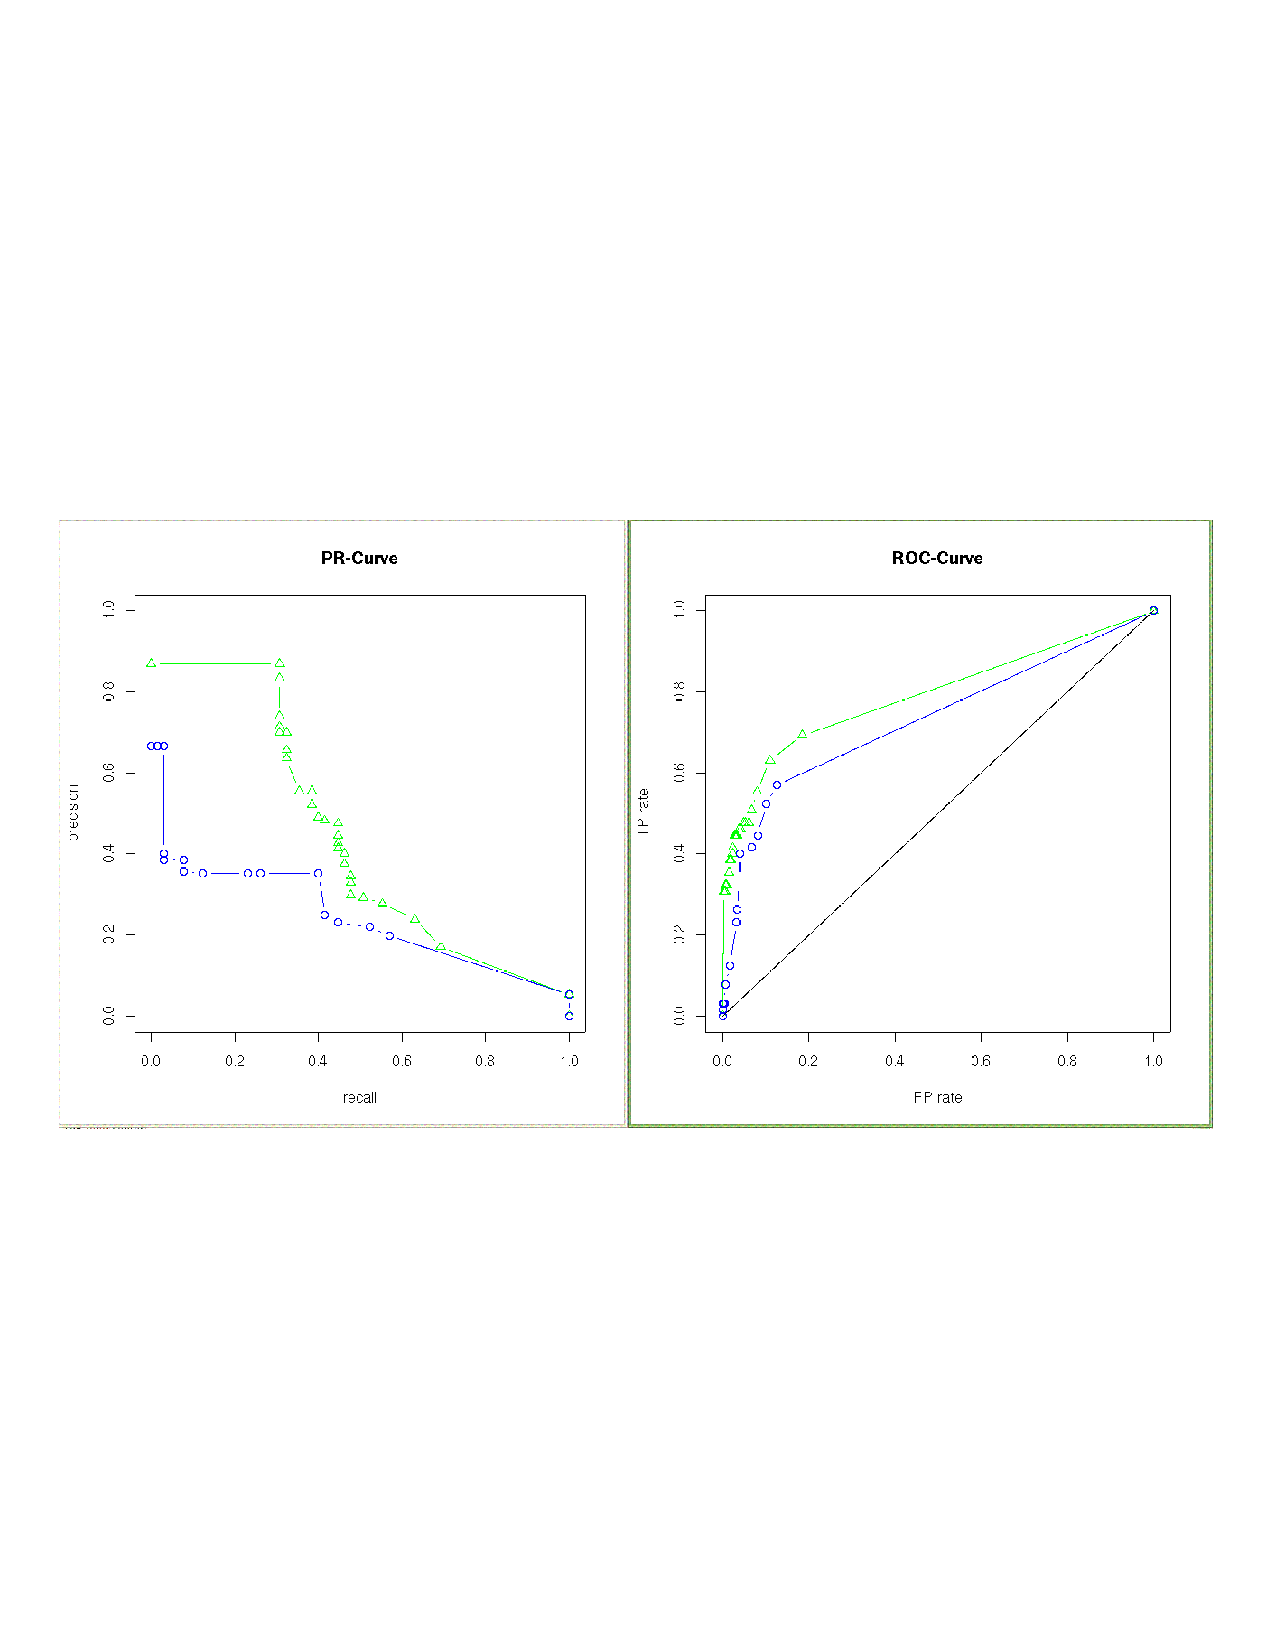
\includegraphics[width=12cm]{courbes}
\caption{Precision-Recall curve (left) and Receiver Operating Characteristic curve (right), 
for both inference algorithms \Robject{mrnet} (green) and \Robject{clr} (blue).}
\end{figure}\end{center}

\subsection{Plotting the infered network with \Rpackage{Rgraphviz}}

In order to plot the infered netwok, we suggest using the \Rpackage{Rgraphviz} 
package with the following code:
\begin{Schunk}
\begin{Sinput}
> library(minet)
> data(syn.data)
> net <- minet(dataset = syn.data, method = "aracne", estimator = "mi.mm")
> n <- list(fillcolor = "lightgreen", fontsize = 20, fontcolor = "red", 
+     height = 0.4, width = 0.4, fixedsize = F)
\end{Sinput}
\end{Schunk}

The above code generates the graph in figure 2.

\newpage
\begin{center}\begin{figure}
\label{fig:graph}
\caption{Infered network plotted using \Rpackage{Rgraphviz}}
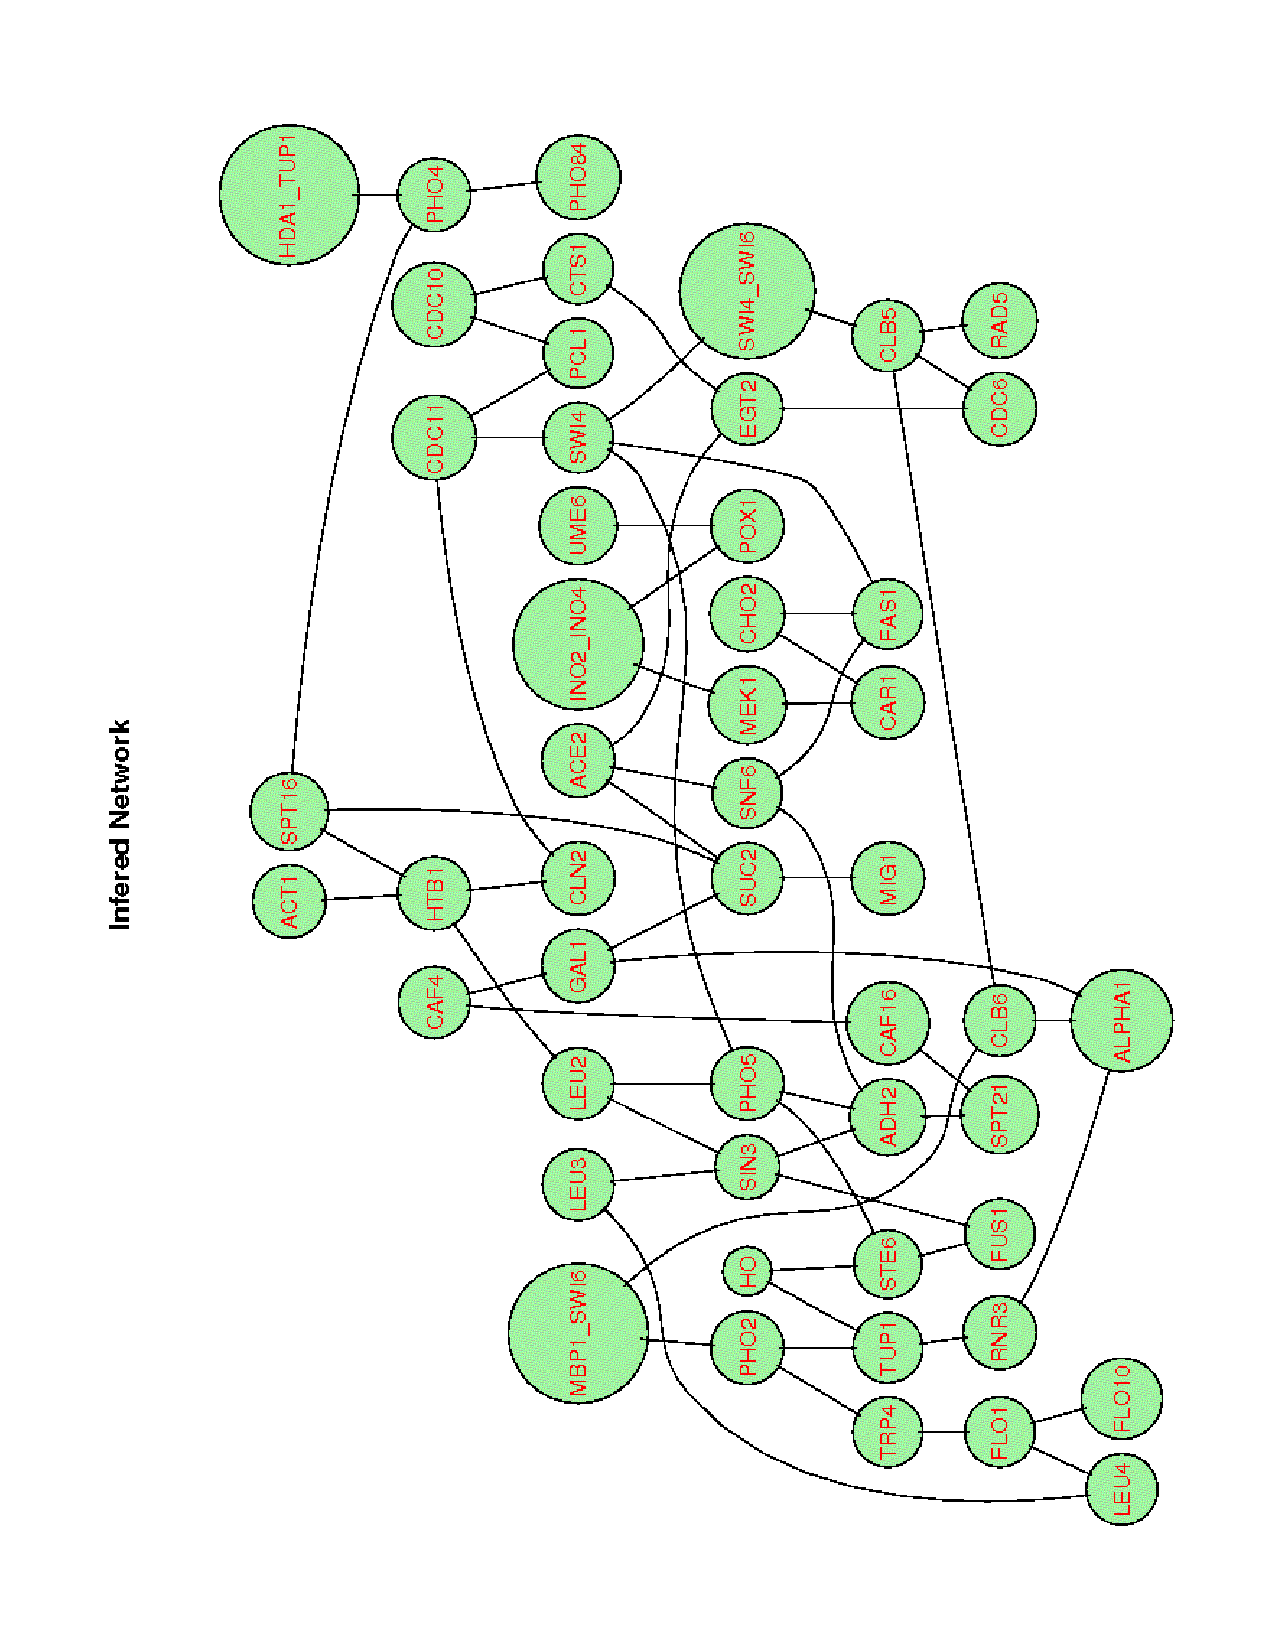
\includegraphics[width=10cm,angle=270]{graph}
\end{figure}\end{center}
\newpage


\bibliographystyle{plain}

\bibliography{minet}

\nocite{*}
\end{document}
